\documentclass[a4paper, 11pt, oneside]{article}

\usepackage[utf8]{inputenc}
\usepackage[T1]{fontenc}
\usepackage[french]{babel}
\usepackage{array}
\usepackage{shortvrb}
\usepackage{listings}
\usepackage[fleqn]{amsmath}
\usepackage{amsfonts}
\usepackage{fullpage}
\usepackage{enumerate}
\usepackage{graphicx}             % import, scale, and rotate graphics
\usepackage{subfigure}            % group figures
\usepackage{alltt}
\usepackage[hidelinks]{hyperref}
\hypersetup{
	colorlinks=true,
	linkcolor=blue,
	filecolor=magenta,
	urlcolor=cyan,
	pdfpagemode=FullScreen,
}
\usepackage{url}
\usepackage{indentfirst}
\usepackage{eurosym}
\usepackage{listings}
\usepackage{color}
\usepackage[table,xcdraw,dvipsnames]{xcolor}

% Change le nom par défaut des listing
\renewcommand{\lstlistingname}{Extrait de Code}

\definecolor{mygray}{rgb}{0.5,0.5,0.5}
\newcommand{\coms}[1]{\textcolor{MidnightBlue}{#1}}

\lstset{
    language=C, % Utilisation du langage C
    commentstyle={\color{MidnightBlue}}, % Couleur des commentaires
    frame=single, % Entoure le code d'un joli cadre
    rulecolor=\color{black}, % Couleur de la ligne qui forme le cadre
    stringstyle=\color{RawSienna}, % Couleur des chaines de caractères
    numbers=left, % Ajoute une numérotation des lignes à gauche
    numbersep=5pt, % Distance entre les numérots de lignes et le code
    numberstyle=\tiny\color{mygray}, % Couleur des numéros de lignes
    basicstyle=\tt\footnotesize,
    tabsize=3, % Largeur des tabulations par défaut
    keywordstyle=\tt\bf\footnotesize\color{Sepia}, % Style des mots-clés
    extendedchars=true,
    captionpos=b, % sets the caption-position to bottom
    texcl=true, % Commentaires sur une ligne interprétés en Latex
    showstringspaces=false, % Ne montre pas les espace dans les chaines de caractères
    escapeinside={(>}{<)}, % Permet de mettre du latex entre des <( et )>.
    inputencoding=utf8,
    literate=
  {á}{{\'a}}1 {é}{{\'e}}1 {í}{{\'i}}1 {ó}{{\'o}}1 {ú}{{\'u}}1
  {Á}{{\'A}}1 {É}{{\'E}}1 {Í}{{\'I}}1 {Ó}{{\'O}}1 {Ú}{{\'U}}1
  {à}{{\`a}}1 {è}{{\`e}}1 {ì}{{\`i}}1 {ò}{{\`o}}1 {ù}{{\`u}}1
  {À}{{\`A}}1 {È}{{\`E}}1 {Ì}{{\`I}}1 {Ò}{{\`O}}1 {Ù}{{\`U}}1
  {ä}{{\"a}}1 {ë}{{\"e}}1 {ï}{{\"i}}1 {ö}{{\"o}}1 {ü}{{\"u}}1
  {Ä}{{\"A}}1 {Ë}{{\"E}}1 {Ï}{{\"I}}1 {Ö}{{\"O}}1 {Ü}{{\"U}}1
  {â}{{\^a}}1 {ê}{{\^e}}1 {î}{{\^i}}1 {ô}{{\^o}}1 {û}{{\^u}}1
  {Â}{{\^A}}1 {Ê}{{\^E}}1 {Î}{{\^I}}1 {Ô}{{\^O}}1 {Û}{{\^U}}1
  {œ}{{\oe}}1 {Œ}{{\OE}}1 {æ}{{\ae}}1 {Æ}{{\AE}}1 {ß}{{\ss}}1
  {ű}{{\H{u}}}1 {Ű}{{\H{U}}}1 {ő}{{\H{o}}}1 {Ő}{{\H{O}}}1
  {ç}{{\c c}}1 {Ç}{{\c C}}1 {ø}{{\o}}1 {å}{{\r a}}1 {Å}{{\r A}}1
  {€}{{\euro}}1 {£}{{\pounds}}1 {«}{{\guillemotleft}}1
  {»}{{\guillemotright}}1 {ñ}{{\~n}}1 {Ñ}{{\~N}}1 {¿}{{?`}}1
}

%%%%%%%%%%%%%%%%% TITRE %%%%%%%%%%%%%%%%
% Complétez et décommentez les définitions de macros suivantes :
 \newcommand{\intitule}{Five or More}
 \newcommand{\GrNbr}{24}
 \newcommand{\PrenomUN}{Timothy}
 \newcommand{\NomUN}{Smeers}
 \newcommand{\PrenomDEUX}{Martin}
 \newcommand{\NomDEUX}{NoirFalise}


%%%%%%%% ZONE PROTÉGÉE : MODIFIEZ UNE DES DIX PROCHAINES %%%%%%%%
%%%%%%%%            LIGNES POUR PERDRE 2 PTS.            %%%%%%%%

\title{INFO0030: \intitule}
\author{Groupe \GrNbr : \PrenomUN~\textsc{\NomUN}, \PrenomDEUX~\textsc{\NomDEUX}}
\date{}

\begin{document}

\maketitle
\newpage
\tableofcontents
\newpage
%%%%%%%%%%%%%%%%%%%% FIN DE LA ZONE PROTÉGÉE %%%%%%%%%%%%%%%%%%%%

%%%%%%%%%%%%%%%% RAPPORT %%%%%%%%%%%%%%%
% Écrivez votre rapport ci-dessous.

% GUI %
\section{GUI}
La GUI est gérée en plusieurs parties, ces parties sont gérées indépendemment les unes des autres. Chaque zone est gérée logiquement dans le modèle et gérée visuellement dans la vue. Les deux étant controlées par le controleur.
(cfr. Figure \ref{fig:zone}).

\begin{itemize}
    \item La zone \textcolor{red}{rouge} contient les menus du programme. Les sous-menu sont liés à des fonctions de callback propres à la vue.
    \item La zone \textcolor{Blue}{bleue} contient les pions de couleurs du prochain tour. Un vecteur fournit une référence vers chacun des boutons permettant de mettre à jour leurs image à chaque tour. \\
    										Cette zone contient également l'affichage du score actualisé à chaques tours.
    \item La zone \textcolor{ForestGreen}{verte} contient le grille de jeu. Une matrice des boutons conserve une référence vers chacun des boutons du tableau de jeu, cela permet de mettre à jour leur image lors d'un déplacement des pions par le joueur.
\end{itemize}

\begin{figure}[h]
    \centering
    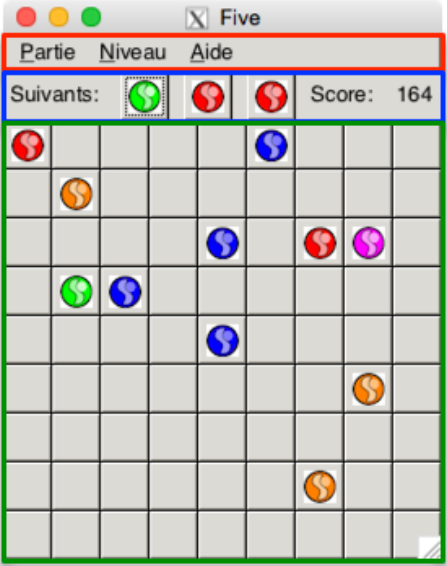
\includegraphics[width=0.4\textwidth]{images/zone.png}
    \caption{Groupements dans la fenêtre}
    \label{fig:zone}
\end{figure}

\section{Structures de Données}
\subsection{modele.c}
\subsubsection{Struct Modele\_t}
Cette structure contient toute les données utiles à la gestion globale du jeu.
\subsection{vue.c}
\subsubsection{Struct Vue\_t}
Cette structure contient en même temps la structure du modèle pour pouvoir avoir accès à toutes les données de jeu. Et contient également la matrice des boutons présents dans la grille, mais aussi les boutons suivants et le score à afficher sur la GUI
\subsection{controleur.c}
\subsubsection{Struct Controler\_t}
Cette structure contient les deux structures, Modele\_t et Vue\_t.
\subsubsection{Struct Data\_tab\_t}
Cette structure contient les informations de la grille permettant de crer des g\_signal\_connect();
\subsection{utils.c}
Ce fichier contient tout les algorithmes simples et de conversion utiles dans plusieurs fichiers sources.

% Algorithmes %
\section{Algorithmes}
Lors de l'élaboration de ce projet, nous avons développé plusieurs algorithmes complexes.
\begin{itemize}
    \item L'algorithme de recherche A*.
    \item Algorithme de répartition aléatoire.
    \item Algorithme de suppression des pions gagnants.
\end{itemize}
\subsection{Algorithme de recherche A*}
L'algorithme de recherche A* est construit sur base de la récursivité et va prendre une à une les cases disponibles aux alentours jusqu'à atteindre (ou pas) la case d'arrivée en contournant les obstacles

\subsection{Algorithme de répartitions aléatoires}
Cet algorithme permet de tirer au hasard un nombre entre 1 et le nombre de cases vides restantes dans la grille de jeu pour ensuite les répartir dans cette même grille.\par
Le nombre de pions à placer dépend du niveau de jeu choisi :
\begin{itemize}
	\item[] 3 pour le niveau ``facile''.
	\item[] 3 pour le niveaux ``moyen''.
	\item[] 7 pour le niveaux ``difficile''.
\end{itemize}
Une fois ces pions placés dans la grille, nous nous devons de réduire la taille du vecteur représentant les cases libres à sa nouvelle valeur.

\subsection{Algorithme de suppression des pions gagnants}
Le but de cet algorithme est de supprimer les pions qui ont permis l'incrémentation du score.\par
Une fois les pions supprimés, nous nous devons d'actualiser la taille du vecteur représentant les cases libres à sa nouvelle valeur.

% Profiling du Code et Analyse de Performance %
\section{Profiling du Code et Analyse de Performance}
Après un profiling, à l'aide de GProf, de notre exécutable,

\begin{itemize}
    \item Les deux fonctions les plus appelées sont (int /char*) et leur complexité est très légère.
    \item Elles sont appelées énormément de fois.
\end{itemize}

% Interface Graphique GUI %
\section{Interface Graphique GUI}
L'interface est illustrée dans les figures :\par \ref{fig:petit}, \ref{fig:moyen}, \ref{fig:difficile}, \ref{fig:end}, \ref{fig:partie}, \ref{fig:niveau}, \ref{fig:aide}, \ref{fig:score}, \ref{fig:a_propos}
\begin{figure}[!h]
    \centering
    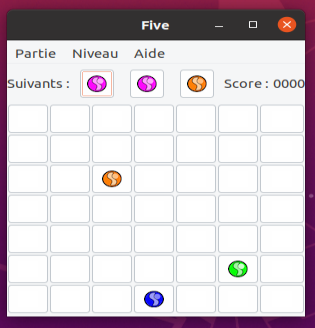
\includegraphics[width=0.4\textwidth]{images/petit.png}
    \caption{Interface de départ pour un niveau facile.}
    \label{fig:petit}
\end{figure}

\begin{figure}[!h]
    \centering
    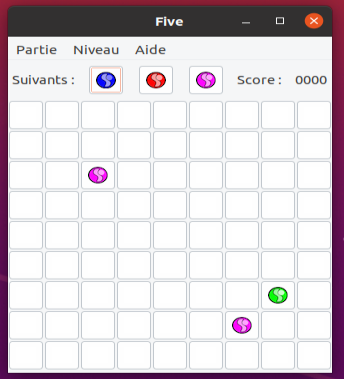
\includegraphics[width=0.4\textwidth]{images/moyen.png}
    \caption{Interface de départ pour un niveau moyen.}
    \label{fig:moyen}
\end{figure}

\begin{figure}
    \centering
    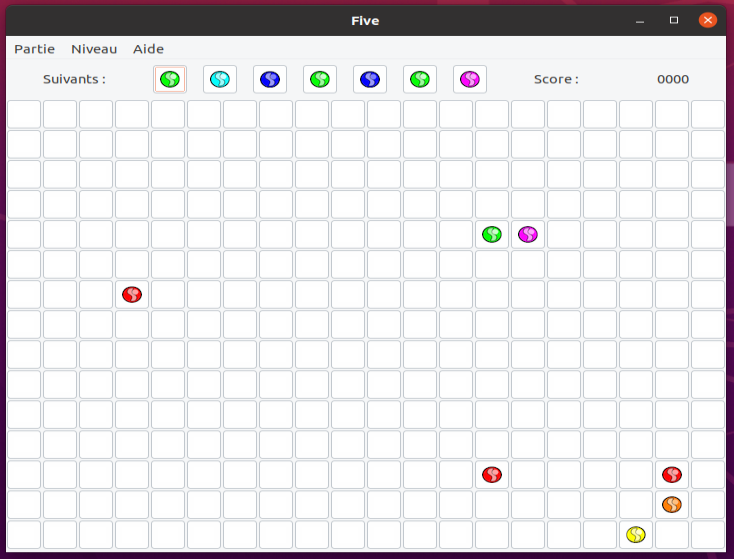
\includegraphics[width=0.4\textwidth]{images/grand.png}
    \caption{Interface de départ pour un niveau difficile.}
    \label{fig:difficile}
\end{figure}

\begin{figure}
    \centering
    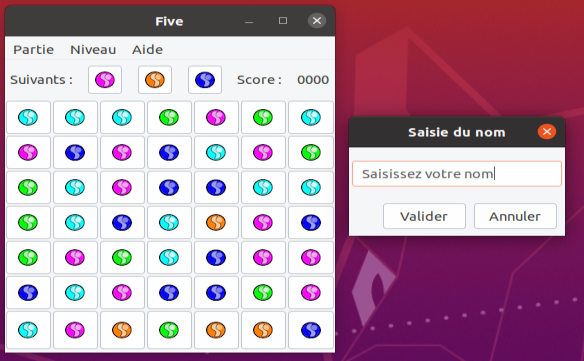
\includegraphics[width=0.4\textwidth]{images/end.png}
    \caption{Interface de fin lorsque le jeu est terminé, nous devons renseigner notre nom.}
    \label{fig:end}
\end{figure}

\begin{figure}
    \centering
    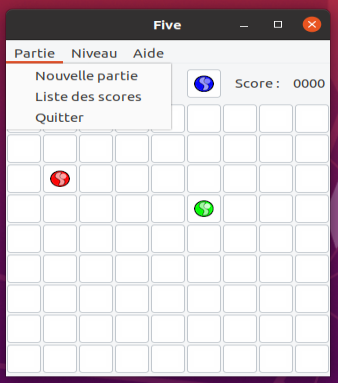
\includegraphics[width=0.4\textwidth]{images/partie.png}
    \caption{Interface du menu de partie. L'utilisateur peut recommencer une nouvelle partie ,quitter le jeu ou consulter les scores.}
    \label{fig:partie}
\end{figure}

\begin{figure}
    \centering
    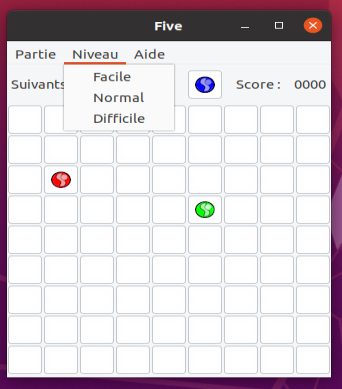
\includegraphics[width=0.4\textwidth]{images/niveau.png}
    \caption{Interface du menu niveau. L'utilisateur peut sélectionner un niveau.}
    \label{fig:niveau}
\end{figure}

\begin{figure}
    \centering
    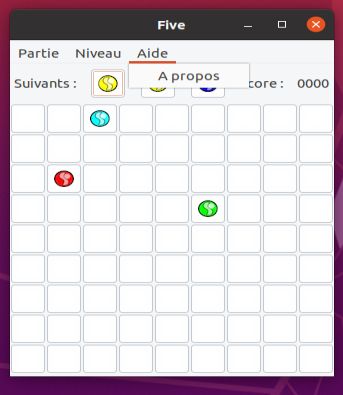
\includegraphics[width=0.4\textwidth]{images/aide.png}
    \caption{Interface du menu d'aide. L'utilisateur peut sélectionner les crédits.}
    \label{fig:aide}
\end{figure}

\begin{figure}
    \centering
    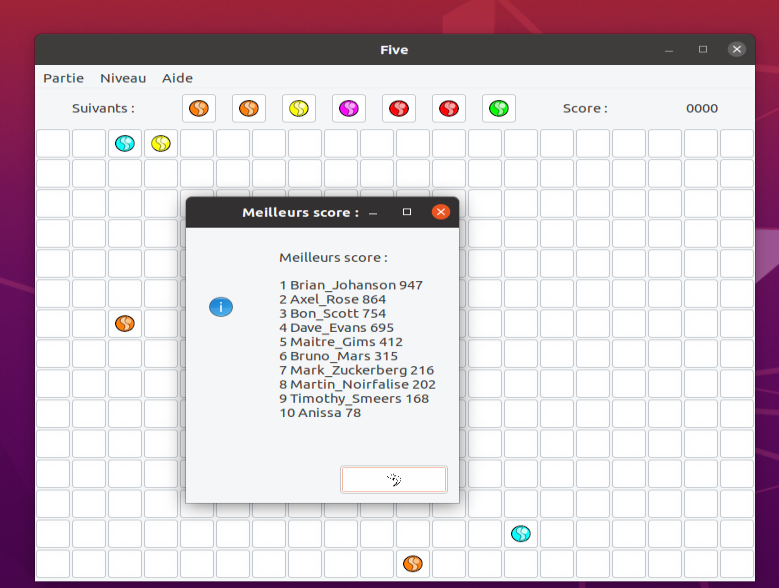
\includegraphics[width=0.4\textwidth]{images/score.png}
    \caption{Interface du pop-up de score. L'utilisateur peut visualiser les meilleurs scores.}
    \label{fig:score}
\end{figure}

\begin{figure}
    \centering
    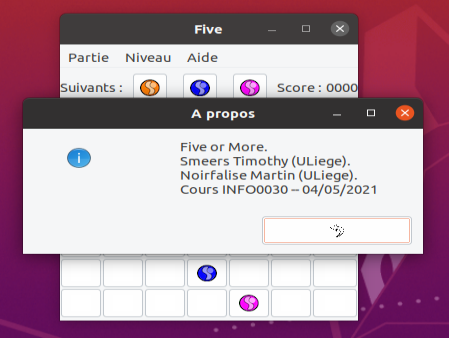
\includegraphics[width=0.4\textwidth]{images/a_propos.png}
    \caption{Interface du pop-up "à propos". L'utilisateur peut consulter les crédits.}
    \label{fig:a_propos}
\end{figure}

\newpage

% Gestion du code %
\section{Gestion du code}
Lors de la réalisation de notre projet, nous avons directement utilisé Un SCM (Git) pour pouvoir travailler en même temps sur des fichiers en parallèle.\par
Le concept du SCM nous étant familier, nous n'avons pas eu de mal à nous en servir.\par
La gestion de tickets et de branches étant très utiles, nous avons jugé bon de nous en servir au maximum avant de commencer à faire des merge-request.

% Coopération au sein du groupe %
\section{Coopération au sein du groupe}
La coopération au sein de notre groupe à été très fructueuse et partagée. Nous ne pouvons pas préciser exactement les taches que nous avons chacun réalisées séparément. Mais nous avons travaillé de différentes façons.\par
\subsection{Martin}
Création de la VBox principale avec tous les menus et la grille.
Élaboration des algorithmes.
\subsection{Timothy}
Déboguage et refactoring du code.
Création des pop-up et algorithmes liés à la barre de menu.
\subsection{Commun}
Les tâches communes ont été très nombreuses avec quelques ``Brain-Stormings'' avant de commencer un nouveaux ticket pour mettre au point notre approche pour l'élaboration du programme.

% Améliorations du programme %
\section{Améliorations du programme}
Si nous avions disposé d'un peu plus de temps nous aurions:\par
\begin{itemize}
    \item Ajouté un meilleur algorithme de traitement des meilleurs scores.
    \item Ajout de différents pop-up's permettant de personnaliser la fenêtre de jeu.
    \item Algorithme A* beaucoup plus élaborer.
    \item Création de pions bonus permettant de supprimer plusieurs pions autours (tel une bombe).
\end{itemize} 

% Apprentissage %
\section{Apprentissage}
Ce projet nous a permis à tout les deux de pouvoir évoluer en groupe pour faire évoluer notre capacité à nous adapter à l'autre.
Ce projet étant assez volumineux nous avons compris l'importance du déboguage et de la programmation défensive.
Bien entendu ceci nous à permis d'apprendre à nous documenter d'une manière plus rigoureuse sur les librairies utilisées utiles à l'élaboration d'algorithmes.

% Documentation %
\section{Documentation}
	Pour plus d'informations sur le code vous pouvez consulter le \href{html/index.html}{site internet} contenant la documentation doxygen.
\end{document}
